%\pagenumbering{arabic}
\section{开发技术选择}

\subsection{非关系型数据库 MongoDB}

在答辩系统的开发中,使用了非关系型数据库 MongoDB。非关系型数据库(NoSQL)提供了一种存储和检索数据的机制,该机制的建模方式不是关系数据库中使用的表格关系。这些数据库自20世纪60年代后期就已存在,但直到21世纪初由Facebook,Google和亚马逊等Web 2.0公司引发的流行高潮才获得“NoSQL”绰号。NoSQL数据库在大数据和实时Web应用程序中被使用得越来越多。NoSQL系统有时也被称为“Not only SQL”,以强调它们可能支持类似SQL的查询语言。

关系数据库要求在添加数据之前定义模式。例如,我们可能希望存储有关用户的数据,例如电话号码、姓名、地址、城市和省份,SQL数据库需要提前知道正在存储的内容。这与适应敏捷开发的理念相悖,因为每次完成新功能开发时,数据库的架构通常都需要更改。例如,如果我们决定对开发进行一些迭代,除了地址和电话号码之外,我们还想存储客户喜欢的商品,则需要将该列添加到数据库,然后将整个数据库迁移到新的模式。如果数据库很大,这是一个非常缓慢的过程,包括很长的停机时间。如果我们经常更改应用程序存储的数据 —— 因为正在快速迭代,此宕机时间可能也会频繁发生。并且使用关系数据库也无法事先有效地处理完全没有结构化或未知的数据。

与关系数据库相比,NoSQL数据库具有更高的可扩展性,并提供卓越的性能,其数据模型解决了关系模型无法解决的几个问题:大量可快速变化的结构、半结构化和非结构化数据;敏捷开发、快速模式迭代以及更频繁的代码推送;面向对象的编程,灵活且易于使用;可在地理上分布式横向扩展架构,而不是使用昂贵的单片架构。

MongoDB是一个免费且开放源码的的数据库程序,跨平台并面向文档,使用类似JSON的文档和模式,因此可以在 JavaScript 中很方便的存储和操作。这意味着字段可能因文档而异,数据结构可能随时间而改变。MongoDB 数据库中的文档模型可以被驱动程序简单地映射为面向对象编程语言中的对象,使数据非常易于使用。

\begin{lstlisting}[title=代码 3-1:“面向对象”的数据库操作示例]
import { Meteor } from 'meteor/meteor';
import {   db   } from '../lib/collections';

let stu = db.users.findOne(ID_OF_THE_STUDENT);

bootbox.confirm(`确定要删除对 ${stu.name} 的评审吗?`, (yes)=>{
	if(!yes) return;
	db.partnership.update(stu._id, {$unset: {
		review_teaname: "",
		review_grades:  "",  
		review_remark:  "",
	}});
	bootbox.alert('评审数据删除完毕');
});
\end{lstlisting}

如代码3-1所示,如果说传统的SQL是“面向过程”的,那么非关系型数据库则是“面向对象”的。第4行中,我们对数据库db的成员变量users集合调用其方法findOne,获得目标学生对象。接下来,在partnership集合中,使用update方法将该学生的3条字段清空。

可以看到,使用MongoDB面向对象的数据操作方式,不仅使源代码更加清晰易懂,也使得项目开发速度远高于传统的“拼装SQL语句”方法。

\begin{lstlisting}[title=代码 3-2:MongoDB 中学生和教师的数据示例]
{   // 学生数据
	"_id" : 	 			"6FXQebx2JBidJZCPo",
	"createdAt" : 			ISODate("2017-12-03T02:02:02.098Z"),
	"username" : 			"201412345678",
	"name" : 				"胡中元",
	"spr_name" : 			"计算机科学与技术",
	"class_name" : 			"计1401",
	"stu_year" : 			2018,
	"spr_id" : 				"tqGWQTZhpFFF7eXqH",
	"class_id" : 			"Q6nm86L8w9AxcsmPP",
	"kind" : 				80,
	"stu_status" :  		300
}
{   // 教师数据
	"_id" : 				"dYkZthDN6ngQucp3n",
	"createdAt" : 			ISODate("2016-11-09T00:35:20.038Z"),
	"username" : 			"123456",
	"name" : 				"张留美",
	"kind" : 				200,
	"is_dean" : 			false,
	"tea_edit_time" : 		ISODate("2018-03-09T04:36:02.408Z"),
	"tea_level" : 			"副教授",
	"inspection_role" : 	2,
	"class_id" : 			"4S4jbXguibvzuWeT9",
	"inspection_group_id" : "PMYxwbCFzySSwxRuZ"
}
\end{lstlisting}

代码3-2中列出的第一个 document 来自一名今年的毕业生(笔者),另一个来自一名今年答辩小组中的教师(笔者的导师)。分别是学生和教师类型的两条数据均存储在同一个 users 集合中,并使用了 kind 字段来划分用户的身份。

可以看见,不同身份的用户拥有的字段部分是相同的,但也有些字段并非如此,比如学生独有的 stu\_status 字段和教师独有的 is\_dean, tea\_level 字段。如果是在关系型数据库中,就需要一个拥有很多字段的表来储存这些不同身份的用户数据,或者是将不同身份的用户保存在不同的表中。然而在 MongoDB 中我们就不用这么麻烦,所有的数据都可以融洽的储存在一起。此外,正是由于这样的特性,我们可以随着系统的开发而有需求性的向已有数据库中新增字段,而非一开始便把数据库结构固定成型,这是传统的关系型数据库所不具备的优点。


\subsection{全栈 JS 开发与前端工程化}

就算是现在,能用 Node 负责全后端的互联网公司也寥寥无几。主要原因是技术较新、人员缺乏,同时不愿放弃已有的成熟的开发经验。而 Node 开发的最大特点就是效率极高(这里指的是运行效率而非开发效率),特别适合超大并发的业务。该答辩系统挑战性地选用了前后端JavaScript语言进行开发,使用同一种语言统一了前后端,开发效率上的好处是不言而喻的。

过去,JavaScript程序员与前端开发人员是同义词,并且始终与浏览器绑定在一起,但这已成为过去。Node.js 的兴起开启了一个新时代。 从那时起,JavaScript 程序员可能不再是限于浏览器的前端开发人员。与其他高级编程语言相比,JavaScript程序员可以在更多的平台上开发。JavaScript 编程语言的相关生态系统在不断的发展。从最初的浏览器到后来的服务器,甚至走得更远 —— 移动应用程序、Bot Frameworks、物联网、3D 游戏甚至虚拟现实都可以使用JavaScript开发。

在介绍前端工程化之前,正如大家所知,Web 开发中有一些独特的特性值得一提:

\begin{enumerate}
	\item 存在一些“开发方言”。浏览器读取的是CSS和JavaScript代码,然而实际上开发者为了使用更多的特性往往会选用一些方言,比如
	SCSS\footnote{SCSS是在 Sass 3.0 版本中引入的新语法,可以被编译或解释为级联样式表(CSS),其语法完全兼容于CSS3,同时还继承了Sass的强大特性。}
	或
	TypeScript\footnote{TypeScript是JavaScript的严格语法超集,并且可选的静态类型被添加到了该编程语言中中。这是由Microsoft发布和维护的一门开源编程语言。}
	,开发完成后再使用相应的工具转换为标准的CSS、JS代码。
	\item 无需编译。前端的主要业务逻辑在 JavaScript 中实现,而 JS 是一门解释型语言,无需编译,这使得代码中的错误只能在运行时被发现,这在项目开发中是致命的。往往需要使用 ESLint 工具对 JS 代码进行审查。
	\item 源代码的可合并性和可压缩性。无论是 HTML 源码还是CSS或JS,都是可以压缩的,压缩后的文件不仅体积更小,可能还会拥有更快的执行速度。并且较小的体积在web开发中可以直接带来更快的页面下载速度,十分重要。类似的,合并多个文件可以减少客户端的HTTP请求数量,有效提高访问速度。
\end{enumerate}

由于这些特性的存在,每次前端开发过程中,我们需要依次进行多个操作:对“方言”进行翻译、代码审查、文件合并、文件压缩。这是非常繁琐的一个过程。

如图3-1所示,本次答辩系统使用了类似 gulp 工具的工程化开发流程。图中以一个 CSS 文件作为示例。在开发者完成代码的编写之后,前端工程化脚本会自动调用SASS工具生成CSS样式,同时检查错误;接下来会合并所有CSS样式,将其压缩。最棒的是接下来会自动在浏览器中完成刷新操作,以供开发者查看最新的页面效果。

\begin{figure}
	\centering
	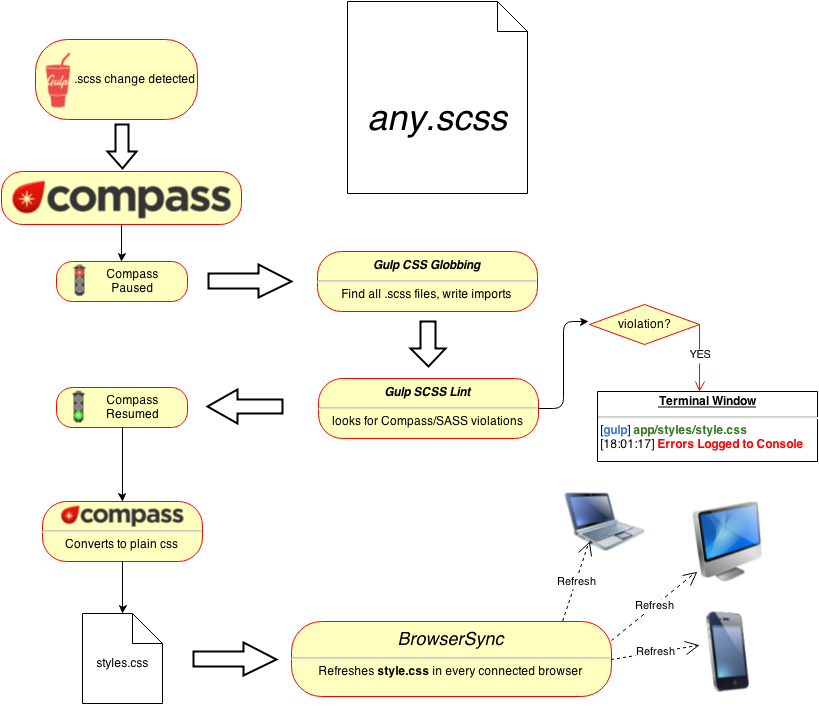
\includegraphics[width=0.85\linewidth]{figure/gulp-flow-scss}
	\caption{gulp 提供的前端开发工作流示例}
\end{figure}

该答辩系统的开发工作流主要由 Meteor 集成。发布应用时,Meteor 会自动将 ES2015 代码编译为浏览器普遍支持的 ES5 代码,并对所有的 CSS 和 JS 进行压缩与合并。在命令界面执行 \textit{meteor run},就会自动执行这一系列操作,并将网页服务运行在 \textit{localhost:3000}。项目运行时,Meteor 也会持续检测代码的变化,会实时地将新的代码加载到浏览器窗口中。


\subsection{Web 高效开发框架 Meteor}

该答辩系统由Meteor框架开发,Meteor是一个现代网站开发框架,基础构架是Node.JS+MongoDB,同时也把这个基础构架从服务器端直接延伸到了浏览器端。这是一个full-stack的JavaScript开发框架,模糊了服务器端和客户端,包括数据库在内的API都可以同时在服务器端和客户端无差异地调用。并且提倡将数据作为前后端交互的内容,而不是HTML网页。配合前端的React框架将来自Meteor的数据渲染成网页,这也是Meteor官方所推荐的组合之一。

在传统的Web应用中,无论是查询数据还是修改数据,任何对数据库的操作都需要客户端向服务端发送一个请求,服务端进行相应的操作,再将结果返回给客户端以供下一步操作。传统的服务器端甚至只充当一个客户端和数据库之间交换数据的中间层。可以说对这样网站的开发,花了相当大的一部分时间在处理请求或处理返回结果上,其实这是多余的过程,Meteor中我们可以直接在客户端中操作数据库,将开发的重点放在业务逻辑上而不是这些重复而花时间的工作上。

\subsubsection{Websocket 通信协议}

WebSocket是一种计算机网络全双工通信的协议,通过单个TCP连接提供了信道。虽然它与HTTP协议不同,但RFC 6455指出WebSocket“通过HTTP端口80和443工作,并支持HTTP代理和中介”,从而使其与HTTP协议兼容。为了实现兼容性,WebSocket握手使用HTTP升级头,让连接从HTTP协议升级为WebSocket协议。

Meteor 和 React 是联合使用的理想选择。两者的特征之一是数据的自动响应 —— Reactivity。这种响应式编程避免了开发者编写代码来跟踪变量更新,因此代码更简单,更易于维护。Meteor使用它自己的基于WebSocket的协议 —— DDP。基本上它使用JSON传递消息。DDP拥有各种主流平台和语言实现。所以将Meteor用作后端服务是完全可行的。

Meteor DDP是一个非常简单上手的协议。DDP可以与任何数据库、框架或编程语言一起工作,并且可以在服务器、客户端和移动设备上工作。实际上,我们可以调用 Meteor.connect() 命令连接到任何DDP服务器,例如其他人编写的Meteor应用程序,并实时订阅其发布的任何数据。

如图3-2所示,利用DDP,Meteor提供了最受欢迎的功能:数据库订阅和服务器端方法。前者使客户端中运行着一个数据库的镜像,而后者使客户现在可以调用我们在服务器上定义的任意JavaScript函数。而无论是数据库订阅还是服务器端方法,其操作权限都是被严格控制的,这在下一节将会具体说明。Meteor也会通过检测重新连接和自动重放缓存,来确保方法只执行一次。

\begin{figure}
	\centering
	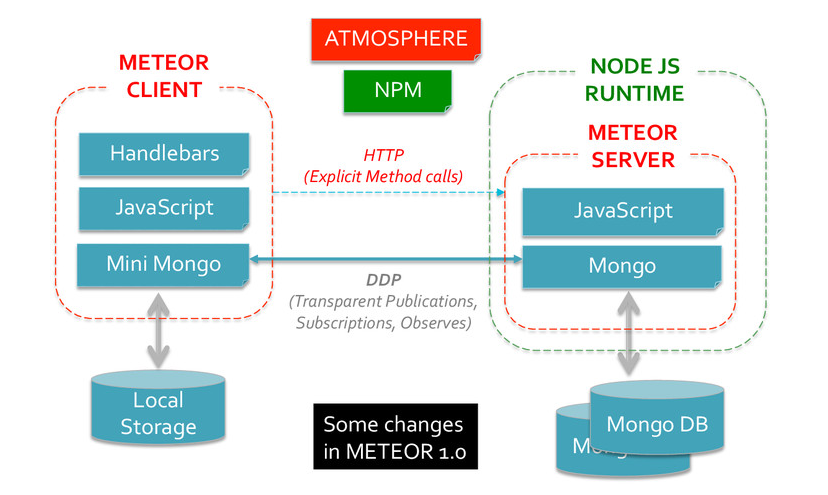
\includegraphics[width=0.85\linewidth]{figure/meteor-logic}
	\caption{Meteor 开发框架逻辑图}
\end{figure}

\subsubsection{权限控制}

然而客户端中直接操作数据库,最让人担心的就是其安全性。在Meteor中,业务逻辑都在客户端中实现,只有一个工作被依然留给了服务器端,那就是对用户权限的鉴定。在服务器端我们可以自由地规定:哪些用户对某个数据库拥有怎样的权限,这样就保证了数据的安全。

在该系统中,feedback集合用于保存用户们的反馈信息。除管理员外的用户能够向其中添加内容,但不能看见其他用户的反馈信息,也只能删除由自己创建的反馈条目。管理员不能进行反馈信息,但可以查看或删除所有用户提交的反馈信息。此外,不对任何角色提供对 feedback 集合中已有条目进行编辑的功能。为了达到这样的需求,定义权限的相关代码如代码3-2所示。

\begin{lstlisting}[title=代码 3-2:Meteor 权限控制示例]
import {Meteor} from 'meteor/meteor';
let db = new Mongo.Collection('feedback');

// define visibilities
Meteor.publish('feedback', function(){
	this.ready();
	
	// get the current user
	let user = Meteor.user() || {};
	
	if(user.kind === 'Admin')
		return db.find();
	else
		return db.find({'user_id': user._id});
});

// define permissions
db.allow({
	'insert': (userId, doc)=>{
		let user = Meteor.user() || {};
		if(user.kind === 'Admin')       return false;
		else if(userId === doc.user_id) return true;
		else                            return false;
	},
	'update': ()=>false,
	'remove': (userId, doc)=>{
		let user = Meteor.user() || {};
		if(user.kind === 'Admin')       return true;
		else if(userId === doc.user_id) return true;
		else                            return false;
	}
});
\end{lstlisting}

通过上面这段定义,对 feedback 数据库需要的权限被我们配置到了服务器端。对于不合法的数据库操作,虽然能够在客户端中尝试进行,但实际上在服务器端是无法对数据库造成任何影响的。总体而言,Meteor 中客户端可以直接方便的读写数据库,同时安全性也被保证。我们可以在同一个文件中规定不同的用户对某个数据库 find、insert、update、remove 四项权限,而不是将判断权限的代码分散在四处,这样让系统变得逻辑清晰、便于维护和开发。


\subsection{React 前端框架}

React(有时称作是React.js或ReactJS)是一个JavaScript库,用于构建用户界面。它由商业公司Facebook和Instagram,以及开源社区中的个人开发人员维护。React可用于开发单页面应用程序和移动应用程序。它主要目的是提供速度,简单性和可扩展性。作为用户界面库,React经常与其他库(如
Redux\footnote{Redux是可预测状态容器,用于JavaScript应用程序中。它可以帮助我们编写React应用程序,该应用程序的支持在不同的环境中运行,行为一致,并且易于调试和测试。最重要的是,它提供了出色的开发者体验,例如结合时间旅行调试器进行的实时代码编辑。}
)结合使用。

如果从MVC框架角度看,React定位在View的范围内。在React 0.14发布之后,React与DOM部分(React-DOM)独立,使React的核心更简单,更符合React的“学习一次,无处不在”的概念。事实上,React的API本身相对简单,但由于整个生态系统非常庞大,因此学习React是一条漫长的道路。React所使用的JSX不是一种全新的语言,而是语法糖,它是一种ECMAScript语法扩展,语法类似于XML。在JSX中,HTML的形成这些元素标签的代码密切相关。

选用React前端框架的优势在于,我们需要一种模块化的技术提高可用性。它可以是一个Web组件,也可以是一个非Web组件。而无论什么样的库或框架,我们都需要某种技术来赋予我们完成抽象、构建和多重复用的能力。而且这个过程不能太繁琐,也不能是一个非常抽象的过程。而React框架为此次答辩系统开发解决了这些问题。

\begin{lstlisting}[title=代码 3-3:React 代码示例]
let fb	= new Mongo.Collection('feedback'),
	dataArray = fb.find({status:0}).fetch();

export default dataArray.map( (item, i)=>(
	<ul key={i}>
		<li>{ item.user_id	}</li>
		<li>{ item.time.toString() }</li>
		<li>{ item.user_tel	}</li>
		<li>{ item.content	}</li>
	</ul>
));
\end{lstlisting}

比如代码3-3所示,读取数据库集合 feedback 中所有来自用户的反馈信息,并返回一组 React components 以供渲染到页面当中。

\begin{enumerate}
	\item 首先创建一个与集合 feedback 的链接,储存在变量 fb 中。
	\item 接着按照 MongoDB 的语法查找出 status 为 0 的文档,使用 fetch 方法转换为数组结构。
	\item 最后使用 JavaScript 中数组对象的 map 方法,返回一个由 React	components 构成的新数组。
\end{enumerate}

在这之后,这一组由反馈信息条目组成的 React  components 就会被我们作为页面组件,按照需要渲染到所需要的页面当中。

虚拟DOM是React非常酷的部分之一。通常情况下,当我们开发具有大量用户交互和数据更新的应用程序时,我们必须仔细考虑应用程序结构对性能的影响。即使使用快速的客户端和先进的JavaScript引擎,广泛的DOM操作也可能成为性能瓶颈,甚至会导致恼人的用户体验。更糟糕的是,由于DOM是树型结构,因此顶层的简单更改可能会导致用户界面的巨大波动。React通过使用虚拟DOM来解决这个问题。顾名思义,这就是对于DOM对象的虚拟表示。任何新的视图更改都首先在虚拟DOM上执行,虚拟DOM位于内存中而不是屏幕上。然后,高效算法将扫描对虚拟DOM所做的更改,以识别需要对真实DOM做出的更改。然后,它确定进行这些更改的最有效方法,最后仅将这些更改应用于真实DOM。这保证了真正DOM的最短更新时间,提供更高的性能和更清晰的用户体验。

考虑到React的优点和缺点,它可以用三个词简单概括:无风险、响应式和先进。这个前端框架背后的主要思想是:“使用随时会发生变化的数据构建大型可伸缩性应用”,并且很好地解决了这个挑战。它为开发人员提供了使用虚拟DOM的能力,而虚拟DOM比真实DOM快得多。除此之外,它还提供了更简单的交互式UI、JSX、基于组件的结构等等。上述因素的结合使其成为Web项目前端开发的合理选择。

